\section{Anzeige Modi}\label{sec_modi}

\ifthenelse{\WCindividualCfg=0 \or \WCmonocolor=0}
{ % generische und RGB color Version des Textes
    \subsection{Einfarb-Modus}\label{sec_modi_monocolor}
				Mit Druck auf die "`\normalModeName"' Taste wird in den 
				\normalModeName gewechselt. 
				
				In diesem wird die Zeit in einer gleichbleibenden Farbe 
				angezeigt.
				\ifthenelse{\WCindividualCfg=0}{
					Handelt es sich bei der WordClock um eine 
					RGB-Version, sind au�erdem folgende Optionen 
					verf�gbar: 
				}{Folgende weitere Optionen sind in diesem Modus verf�gbar:}
				
				\subsubsection{Definierte Farbprofile}
						Es stehen \WCcolorProfiles  Farbprofile zur Verf�gung. Mittels der 
						"`\normalModeName"' Taste kann zwischen den 
						unterschiedlichen Farbprofilen gewechselt werden. 
						
						Die Stundenw�rter zeigen dabei kurzzeitig die Nummer 
						des aktuell ausgew�hlten Profils an. 
						
				\subsubsection{Farbprofil anpassen}
						Die Farbe eines Profils kann ver�ndert werden, indem 
						mittels der Tasten "`Farbe Rot �ndern"', "`Farbe Gr�n 
						�ndern"' oder "`Farbe Blau �ndern"' ein Farbkanal 
						ausgew�hlt wird. Dieser kann dann mittels der "`+/-"' 
						Tasten ver�ndert werden. So kann die Farbe beliebig 
						eingestellt werden. 
						
				\subsubsection{Farbspektrum durchlaufen}
						Alternativ kann man nach Bet�tigung der Taste 
						"`Farben durchschalten"' mittels der "`+/-"' Tasten das 
						Farbspektrum durchlaufen und so eine beliebige Farbe 
						ausgew�hlt werden. 
 
						\begin{Anmerkung}
								Die Spektrumsfarbauswahl wird gegenw�rtig nicht im 
								Farbprofil gespeichert. 
						\end{Anmerkung}
						
						
		\subsection{Automatischer Farbwechselmodus}\label{sec_modi_fade}
				Mit der Taste "`Automatischer Farbwechselmodus"' wird 
				in einen Modus gewechselt, der automatisch langsam 
				das Farbspektrum durchl�uft.
				 
				Mittels der "`+/-"' Tasten kann die Geschwindigkeit des 
				Farbwechsels ver�ndert werden.
				 
				\ifthenelse{\WCindividualCfg=0}{
						\begin{Anmerkung}
								Der automatische Farbwechselmodus ist nur in der 
								RGB"=Version verf�gbar.
						\end{Anmerkung}
			  }
}{% reine Monocolor Version des Textes
    \subsection{Standard-Modus}\label{sec_modi_monocolor}
				Durch Bet�tigung der der gleichnamigen Taste wird in den "`\normalModeName"'
				gewechselt. 
				In diesem wird die Uhrzeit mit einer gleichbleibenden Helligkeit 
				(entsprechend der automatischen Helligkeitssteuerung) angezeigt.
}				

		\subsection{Pulsierender Modus}\label{sec_modi_pulse}
				Dieser Modus kann aus dem \normalModeName
				\ifthenelse{\WCindividualCfg=0 \or \WCmonocolor=0}{ und Farbwechselmodus}{}
				mit der Taste "`Pulsierender Modus"' aktiviert und mit einer 
				weiteren Bet�tigung wieder deaktiviert werden. 
				
				In diesem Modus wird die Helligkeit der Uhr in einem 
				pulsierenden Muster zwischen hell und dunkel ver�ndert. 
				
				Mittels der "`+/-"' Tasten kann die Geschwindigkeit 
				ver�ndert werden. 
				
				\begin{Anmerkung}
						W�hrend dieser Modus aktiv ist, ist die automatische 
						Helligkeitsanpassung deaktiviert. 
				\end{Anmerkung}
				
		\subsection{Demo-Modus}\label{sec_modi_demo}
				Der Demo"=Modus schaltet die Ausg�nge der Reihe nach 
				einzeln an. 
				
				Dieser Modus dient haupts�chlich zum Testen der 
				WordClock"=Schaltung, sowie zur �berpr�fung der 
				richtigen Beschaltung der LED Ausg�nge. 
		
		\subsection{Sprachmodus-Auswahl}\label{sec_modi_regio}
				Mittels der Sprachmodi"=Taste kann zwischen  
				verschiedenen deutschen Formulierungsarten 
				umgeschaltet werden. 
				
				Es stehen folgende 8 Sprachmodi zur Verf�gung: 
				
				\begin{compactenum}
						\item  "`Wessi"'-Modus (st�ndige Anzeige "`Es ist"') 
						\item  "`Wessi"'-Modus  
						\item  "`Rhein-Ruhr"'-Modus (st�ndige Anzeige "`Es ist"') 
						\item  "`Rhein-Ruhr"'-Modus 
						\item  "`Ossi"'-Modus (st�ndige Anzeige "`Es ist"') 
						\item  "`Ossi"'-Modus 
						\item  "`Schwaben"'-Modus (st�ndige Anzeige "`Es ist"') 
						\item  "`Schwaben"'-Modus
				\end{compactenum}
				
				Im Modus 2, 4, 6 und 8 erfolgt die Anzeige "`Es ist"' nur 
				zur halben und vollen Stunde.
				Dies ist um eine allzu ungleiche Leuchtdauer der LEDs zu verhindern 
				und somit ein Voraltern dieser h�ufig benutzten LEDs zu verhindern.
				


					\begin{center}
					  \arrayrulecolor{colorBack}
						\begin{tabular}{|C{.15\textwidth}L{.22\textwidth}L{.22\textwidth}L{.22\textwidth}|}
								\hline
								\rowcolor{colorBack}  {\textcolor{white}{}} 
																		& {\textcolor{white}{6:15}} 
																		& {\textcolor{white}{8:45}} 
																		& {\textcolor{white}{1:20}}\tabularnewline
								\hline
								{Wessi}& {viertel nach sechs}&{viertel vor neun}&{zehn vor halb zwei}\tabularnewline
								\hline
								{Rhein-Ruhr}& {viertel nach sechs }&{viertel vor neun }&{zwanzig nach eins }\tabularnewline
								\hline
								{Ossi}& {viertel sieben}&{dreiviertel neun}&{zehn vor halb zwei}\tabularnewline
								\hline
								{Schwabe}& {viertel sieben}&{dreiviertel neun}&{zwanzig nach eins}\tabularnewline
								\hline
						\end{tabular}
				\end{center}

				 
				\begin{Anmerkung}
						Die Bezeichnung Ossi/Wessi"=Modus ist weder 
						diskriminierend gemeint noch 100\%ig korrekt. Es 
						scheint mehr oder weniger ein breites Band zu sein, 
						das von S�dwest nach Nordost verl�uft, in dem die 
						Ossi"=Variante gesprochen wird. 
						
						Weitergehende Informationen zu den unterschiedlichen 
						Aussprachen findet man im Internet: \\
						\url{http://de.wikipedia.org/wiki/Uhrzeit}\\
						\url{http://www.norddeutschelernendieuhrzulesen.de}
				\end{Anmerkung}
				
				
\begin{figure}[b]
	\centering
		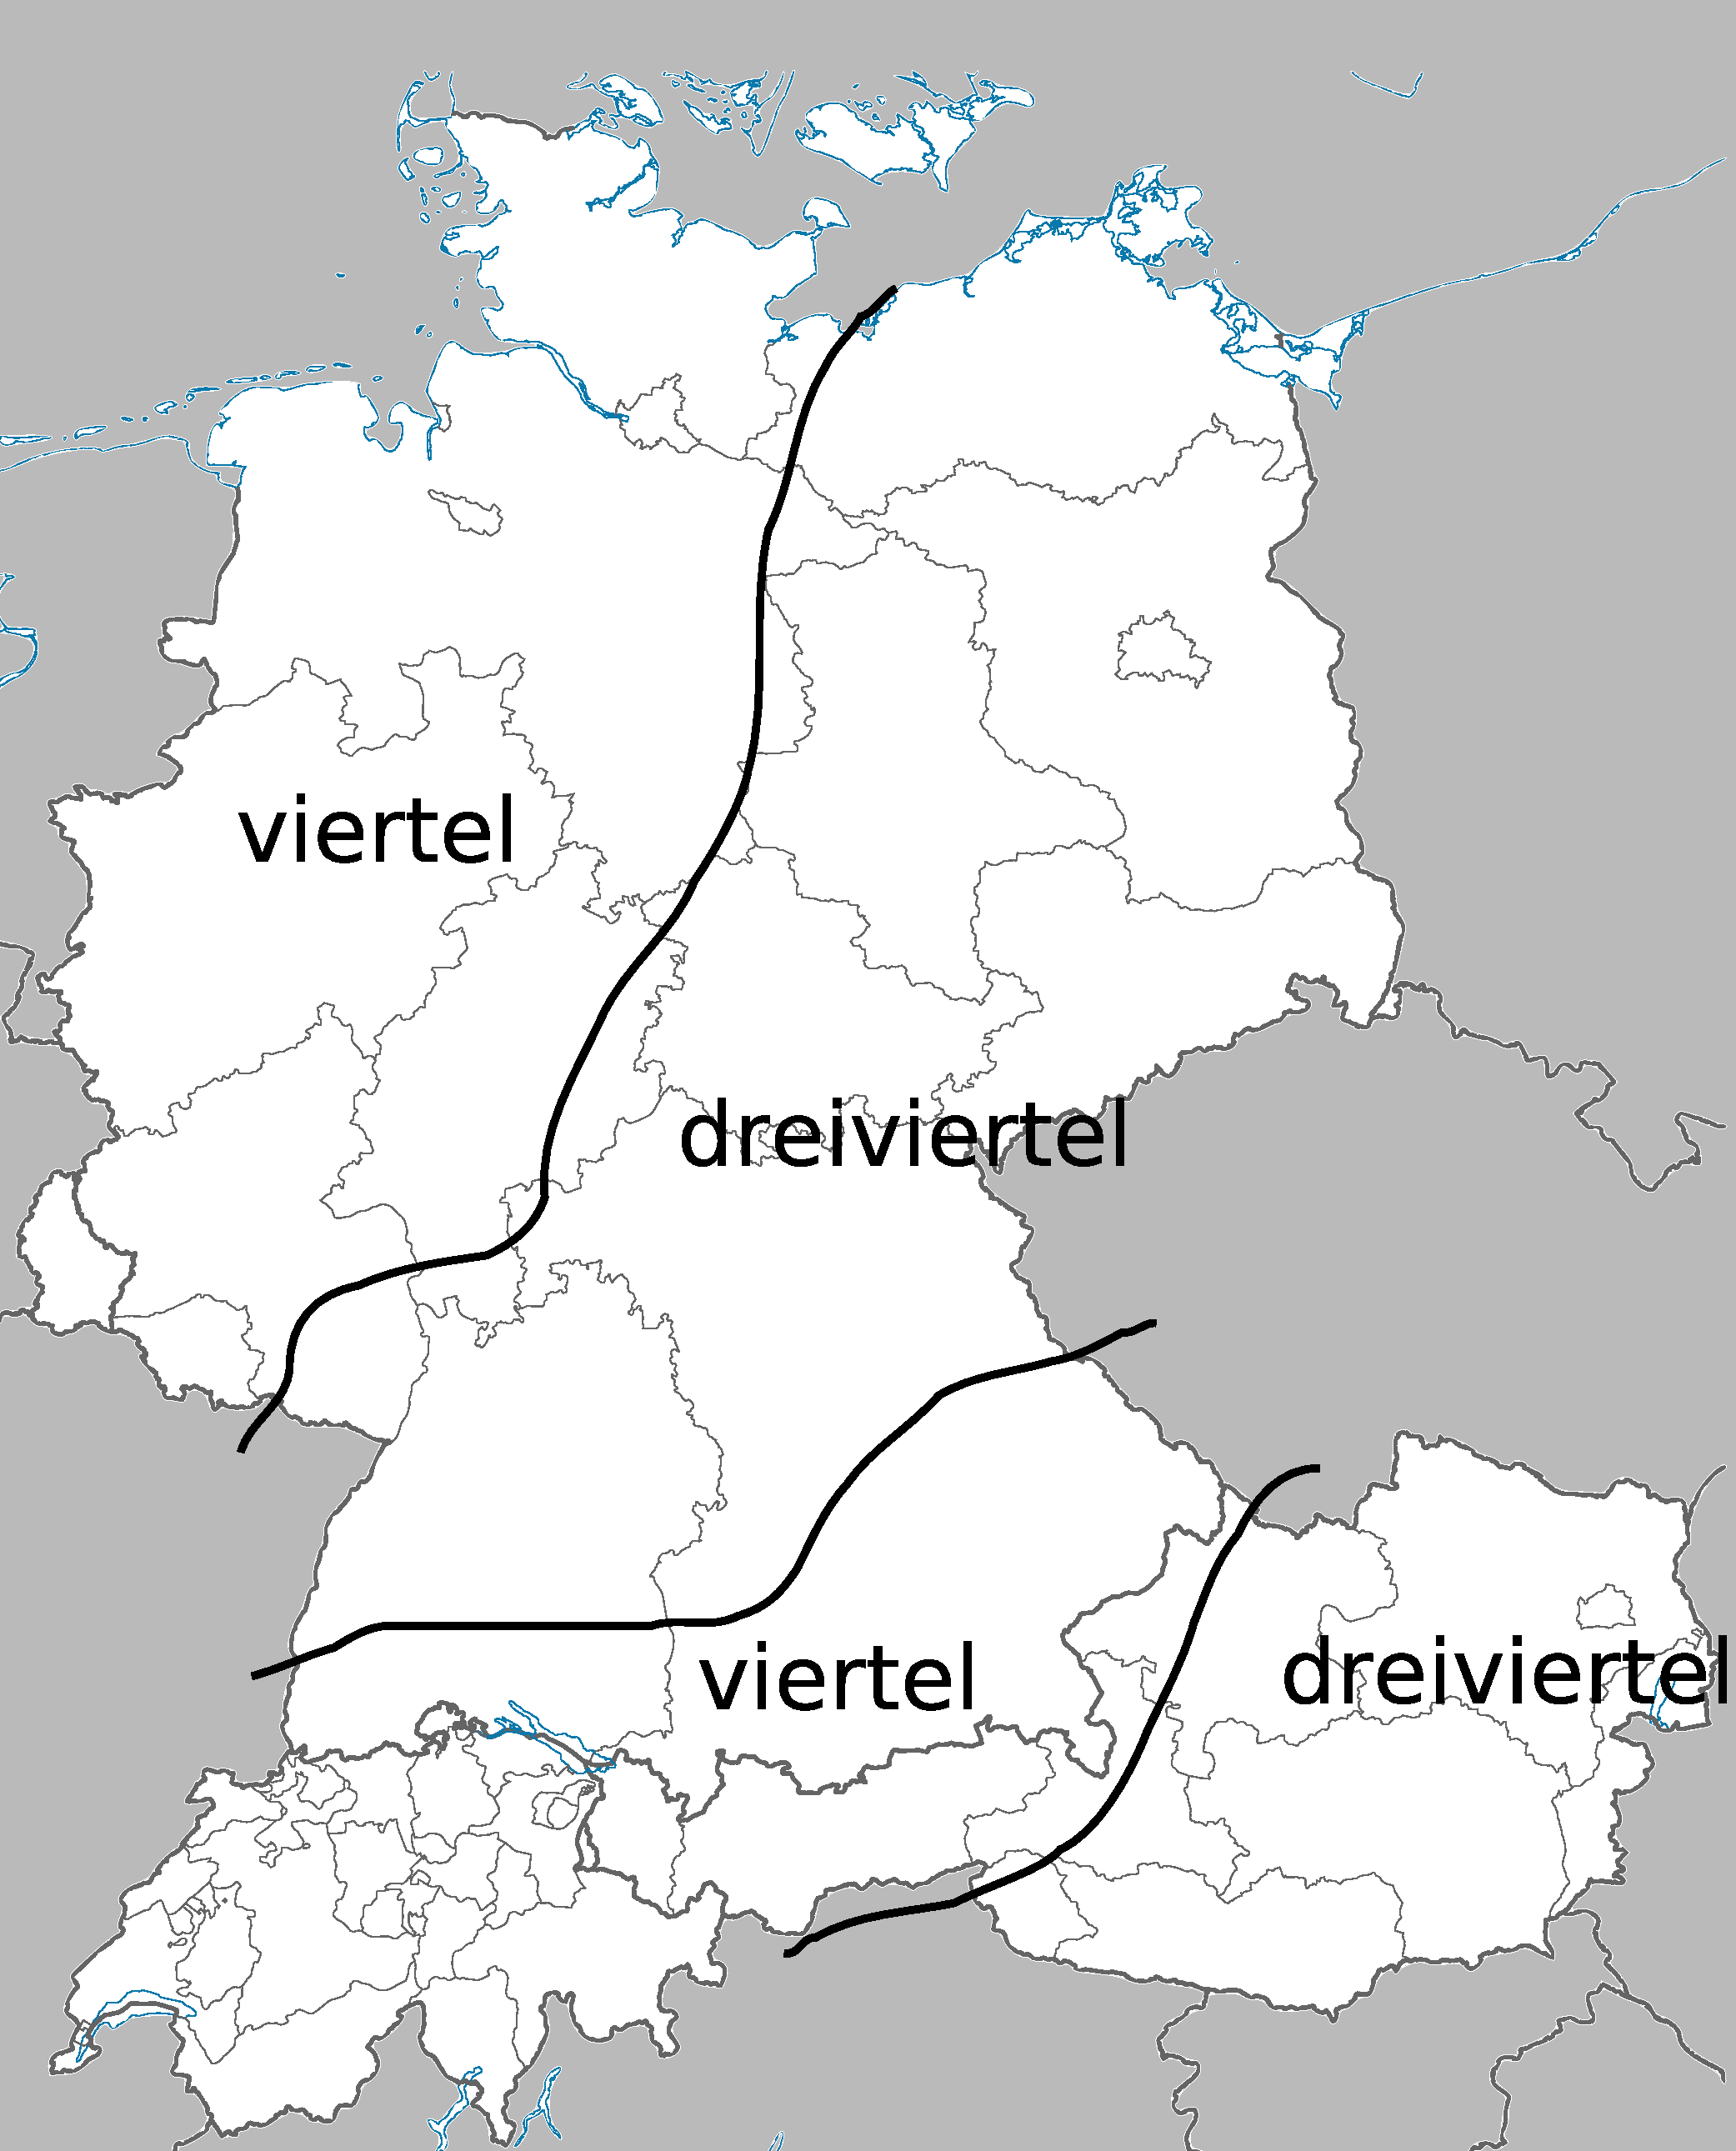
\includegraphics[width=1.00\textwidth]{regiomap.pdf}
	\label{fig:karte}
	\caption{Karte zur Verwendung von "`Dreiviertel"'}
\end{figure}
